\documentclass[10pt,journal]{IEEEtran}
\usepackage[spanish]{babel}
\usepackage[T1]{fontenc}
\usepackage{amsmath}
\usepackage{amssymb}
\usepackage{float}
\usepackage{graphicx}
\usepackage{booktabs}
\usepackage{placeins}
\usepackage{xcolor}
\usepackage{listings}

\lstdefinestyle{consolestyle}{
  language=bash,
  basicstyle=\ttfamily\small,
  breaklines=true,
  showstringspaces=false,
  frame=single,
  framesep=3pt,
  columns=flexible,
}
\lstset{style=consolestyle}
\usepackage[pdfauthor={Jheison Martinez Bolivar},pdftitle={Custom Vision: Animal Identification},colorlinks,linkcolor=blue,citecolor=green,urlcolor=cyan]{hyperref}

\begin{document}

  \title{Custom Vision: Identificaci\'on de Animales\\ Clasificaci\'on con Azure AI Services y Quick Training}

  \author{
    Jheison Martinez Bolivar\\
    \textit{Maestr\'ia en Inteligencia Artificial}\\
    \textit{Universidad de La Salle, Bogot\'a, Colombia}\\
    \texttt{jhmartinez07@unisalle.edu.co}
  }
  \maketitle
  \markboth{Universidad de La Salle --- Aprendizaje de M\'aquina. Noviembre 2026}{}

  \begin{abstract}
    Se construye un clasificador de im\'agenes de elefantes, jirafas y leones con Azure Custom Vision \cite{microsoft_customvision2024} sobre Azure AI Services \cite{microsoft_cognitiveservices2024}. La suscripci\'on Azure for Students impone la policy \texttt{sys.regionrestriction} que solo permite \texttt{francecentral, belgiumcentral, northcentralus, spaincentral, chilecentral}; por ello el instructivo original en \texttt{East US} falla con \texttt{InvalidTemplateDeployment / RequestDisallowedByAzure}. Verificado por CLI, solo \texttt{northcentralus} soporta \texttt{CustomVision.Training} y \texttt{Prediction}, as\'i que los recursos \texttt{labunisalle} y \texttt{labunisalle-Prediction} se crean all\'i en SKU \texttt{S0}. El proyecto \texttt{Animal Identification} es de tipo Classification, Multiclass, dominio General, con 17 im\'agenes por clase y entrenamiento r\'apido. Este borrador documenta hasta el entrenamiento; las m\'etricas, la publicaci\'on y la prueba del cliente se completan cuando el portal entregue los valores.
  \end{abstract}

  \section{Recursos en Azure}

  El grupo \texttt{lab} ya exist\'ia en \texttt{eastus}. El intento del instructivo en \texttt{East US} fue bloqueado por la policy de la suscripci\'on. La evidencia por CLI:

  \begin{lstlisting}
$ az policy assignment show --name sys.regionrestriction
Allowed: francecentral, belgiumcentral, northcentralus,
  spaincentral, chilecentral
$ az cognitiveservices account list-skus \
  --kind CustomVision.Training --location northcentralus
F0, S0
$ az cognitiveservices account list-skus \
  --kind CustomVision.Training --location francecentral
(vacio)
  \end{lstlisting}

  Solo \texttt{northcentralus} devuelve SKUs para Training y Prediction; las otras cuatro regiones permitidas devuelven tabla vac\'ia. Se crearon entonces, en el grupo \texttt{lab}:

  \begin{itemize}
    \item \texttt{labunisalle} --- \texttt{CustomVision.Training}, \texttt{northcentralus}, \texttt{S0}.
    \item \texttt{labunisalle-Prediction} --- \texttt{CustomVision.Prediction}, \texttt{northcentralus}, \texttt{S0}.
  \end{itemize}

  La Figura~\ref{fig:recursos} muestra la creaci\'on en el portal y la Tabla~\ref{tab:recursos} la verificaci\'on por CLI (\texttt{az cognitiveservices account list --resource-group lab}).

  \begin{figure}[H]
    \centering
    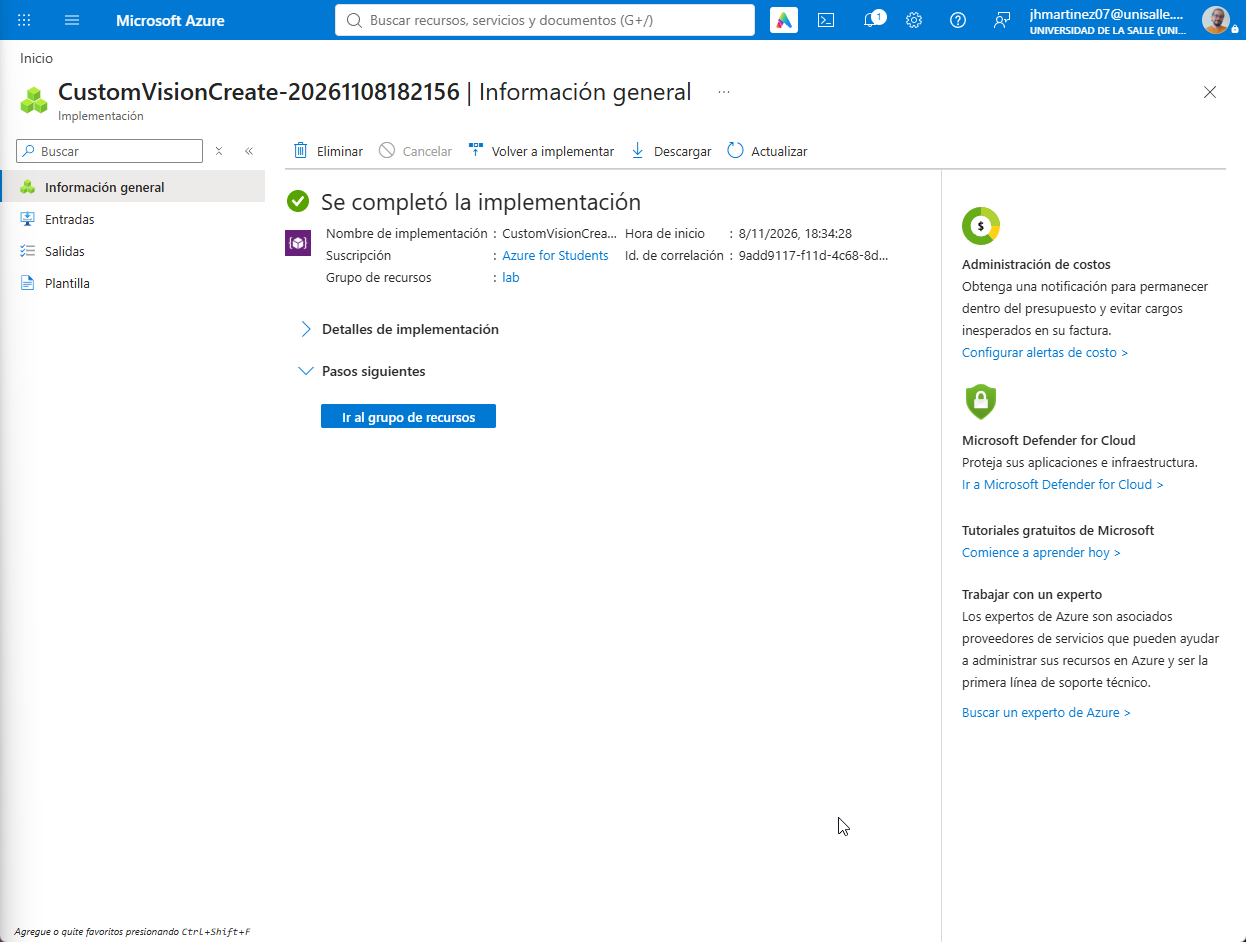
\includegraphics[width=0.9\linewidth]{assets/images/fig_recursos.png}
    \caption{Creaci\'on de los recursos en el portal de Azure.}
    \label{fig:recursos}
  \end{figure}

  \begin{table}[H]
    \centering
    \caption{Recursos verificados por CLI.}
    \label{tab:recursos}
    \begin{tabular}{lll}
      \toprule
      Nombre & Kind & Location / SKU \\
      \midrule
      labunisalle & CustomVision.Training & northcentralus / S0 \\
      labunisalle-Prediction & CustomVision.Prediction & northcentralus / S0 \\
      \bottomrule
    \end{tabular}
  \end{table}

  \section{Proyecto de Custom Vision}

  El recurso no es el proyecto. El proyecto se crea en \texttt{customvision.ai} con el recurso de entrenamiento como contenedor de llaves. Ajustes usados (Figura~\ref{fig:proyecto}):

  \begin{itemize}
    \item Name: \texttt{Animal Identification}.
    \item Description: \texttt{Image classification for animals}.
    \item Resource: \texttt{labunisalle [northcentralus]}.
    \item Project Type: Classification.
    \item Classification Type: Multiclass (Single tag per image).
    \item Domain: General (se documenta si en \texttt{northcentralus} aparece como \texttt{General [A2]} o \texttt{General}).
  \end{itemize}

  \begin{figure}[H]
    \centering
    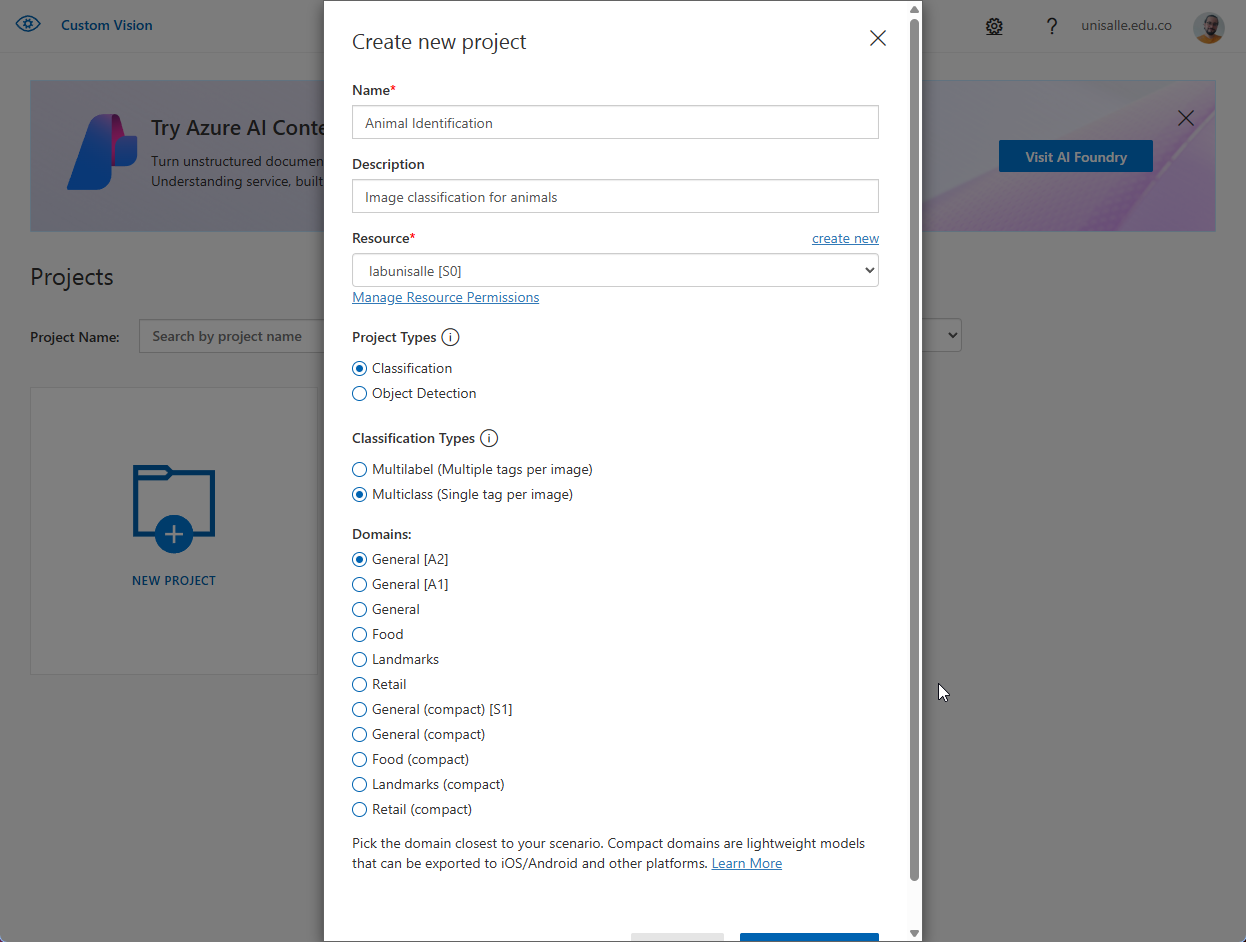
\includegraphics[width=0.9\linewidth]{assets/images/fig_create_project.png}
    \caption{Creaci\'on del proyecto Animal Identification en customvision.ai.}
    \label{fig:proyecto}
  \end{figure}

  \section{Carga y Etiquetado}

  Se descarg\'o el paquete de entrenamiento y se subi\'o por etiquetas: \texttt{elephant}, \texttt{giraffe}, \texttt{lion}, con 17 im\'agenes por clase (Figura~\ref{fig:tags}). Cada lote se etiqueta al subirlo; una imagen con m\'as de una etiqueta romper\'ia el supuesto Multiclass, por eso se verifica un solo tag por imagen.

  \begin{figure}[H]
    \centering
    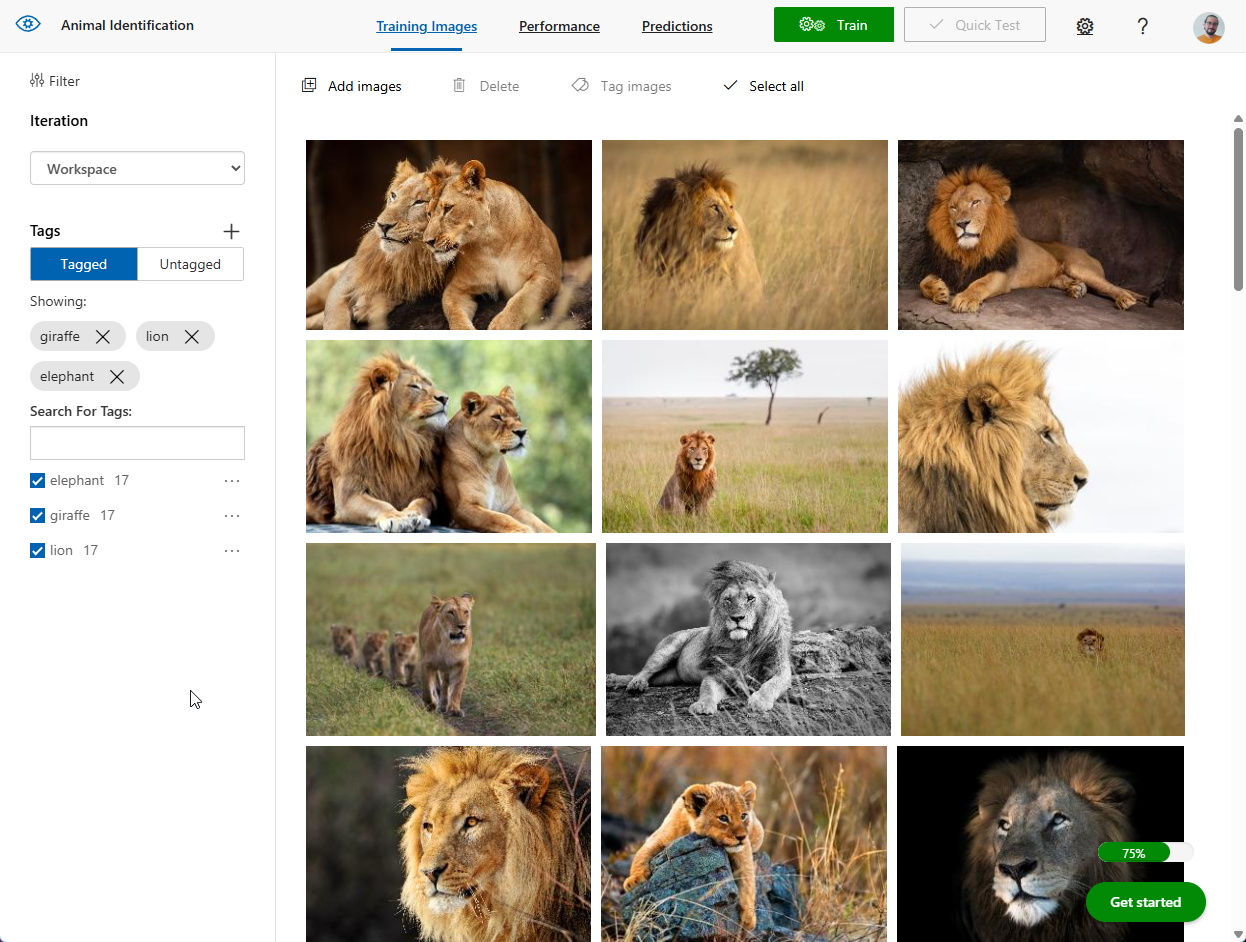
\includegraphics[width=0.9\linewidth]{assets/images/fig_tags.png}
    \caption{Lotes etiquetados por clase, 17 im\'agenes cada uno.}
    \label{fig:tags}
  \end{figure}

  \section{Entrenamiento}

  Se entren\'o con \texttt{Train} en modo Quick Training (Figura~\ref{fig:train}). La Iteraci\'on 1 termin\'o el 8/11/2026 a las 6:51:53 PM con dominio \texttt{General [A2]}, ID \texttt{71779344-fd60-4c43-9e8f-788ef5230282}, tipo Multiclass (Figura~\ref{fig:result}).

  \begin{figure}[H]
    \centering
    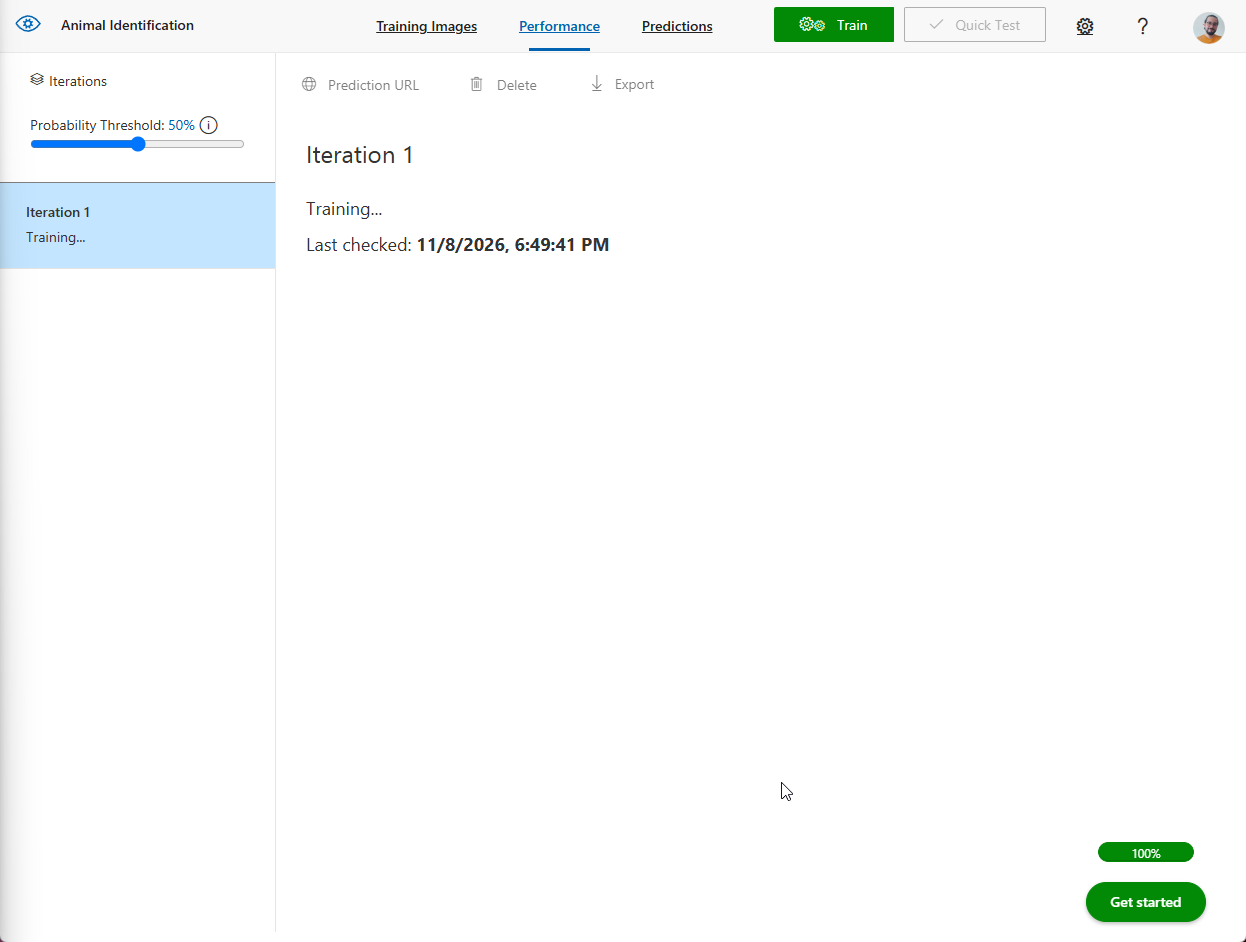
\includegraphics[width=0.9\linewidth]{assets/images/fig_train.png}
    \caption{Entrenamiento r\'apido lanzado y completado.}
    \label{fig:train}
  \end{figure}

  \begin{figure}[H]
    \centering
    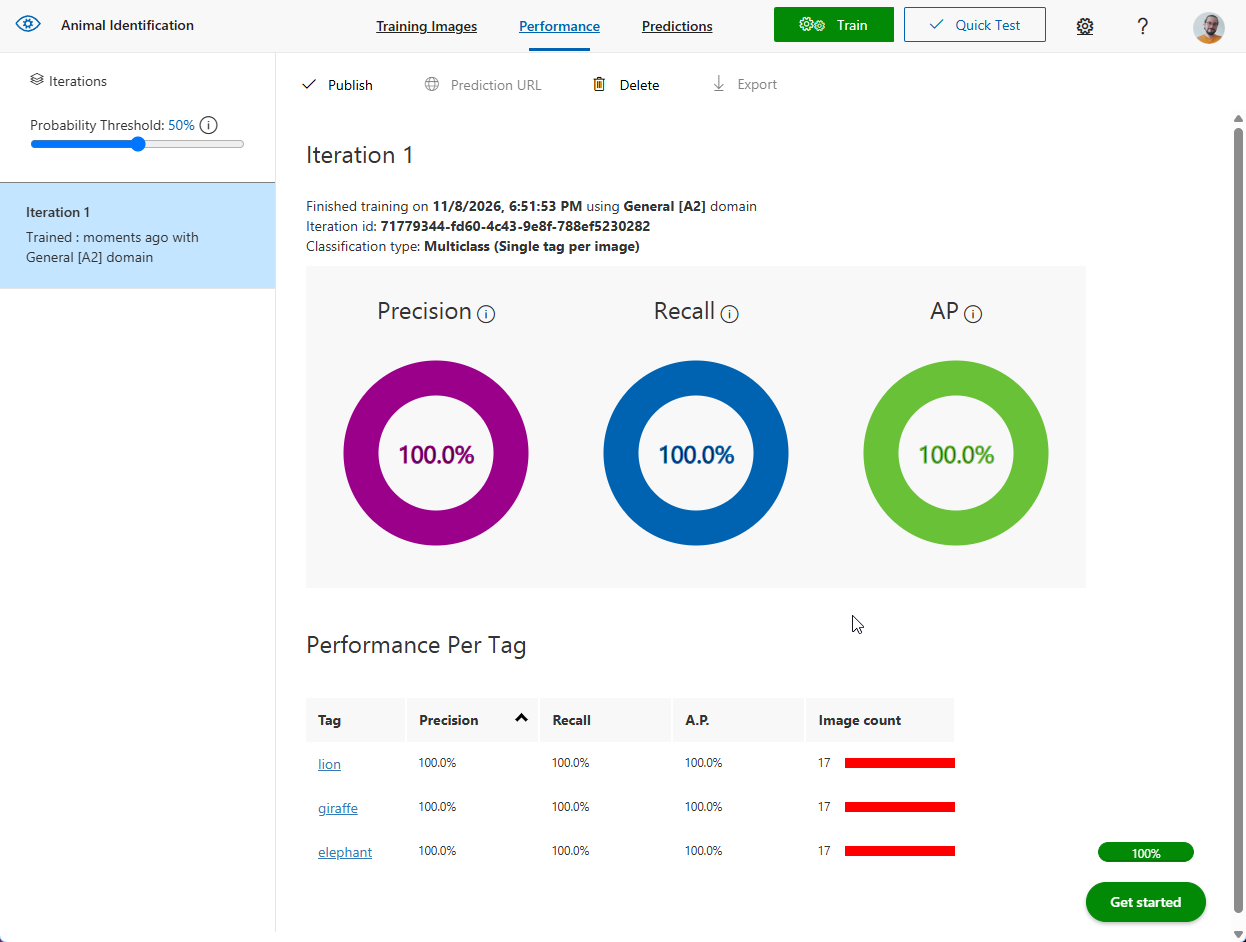
\includegraphics[width=0.9\linewidth]{assets/images/fig_train_result.png}
    \caption{Performance de la Iteraci\'on 1: Precision, Recall y AP globales en 100.0\%.}
    \label{fig:result}
  \end{figure}

  \section{Evaluaci\'on}

  La Tabla~\ref{tab:performance} resume el panel Performance con umbral 50\%. El 100\% en las tres m\'etricas y en los tres tags se lee con cautela: con 51 im\'agenes el modelo memoriza el set de entrenamiento; la prueba que importa es con im\'agenes nuevas.

  \begin{table}[H]
    \centering
    \caption{Performance por tag, Iteraci\'on 1.}
    \label{tab:performance}
    \begin{tabular}{lccc}
      \toprule
      Tag & Precision & Recall & Im\'agenes \\
      \midrule
      lion & 100.0\% & 100.0\% & 17 \\
      giraffe & 100.0\% & 100.0\% & 17 \\
      elephant & 100.0\% & 100.0\% & 17 \\
      \midrule
      Global & 100.0\% & 100.0\% & 51 \\
      \bottomrule
    \end{tabular}
  \end{table}

  Se probaron 6 im\'agenes externas de Wikimedia Commons (carpeta \texttt{validacion/}, con fuentes en \texttt{FUENTES.txt}), no vistas en entrenamiento, con \texttt{Quick Test} sobre la Iteraci\'on 1. La Tabla~\ref{tab:quicktest} y las Figuras~\ref{fig:qt1}--\ref{fig:qt3} muestran que las 6 clasifican bien, con confianza media 96.7\%. El caso m\'as d\'ebil es \texttt{giraffe\_val\_02} (tres jirafas juntas, 87.0\% con 11.4\% a elephant), que es el \'unico con oclusi\'on y m\'ultiples instancias.

  \begin{table}[H]
    \centering
    \caption{Quick Test con im\'agenes nuevas (6/6 aciertos).}
    \label{tab:quicktest}
    \begin{tabular}{lcc}
      \toprule
      Imagen & Predicci\'on correcta & Confianza \\
      \midrule
      elephant\_val\_01 & elephant 98.0\% & 98.0\% \\
      elephant\_val\_02 & elephant 97.6\% & 97.6\% \\
      giraffe\_val\_01 & giraffe 98.5\% & 98.5\% \\
      giraffe\_val\_02 & giraffe 87.0\% & 87.0\% \\
      lion\_val\_01 & lion 99.8\% & 99.8\% \\
      lion\_val\_02 & lion 99.6\% & 99.6\% \\
      \bottomrule
    \end{tabular}
  \end{table}

  \begin{figure}[H]
    \centering
    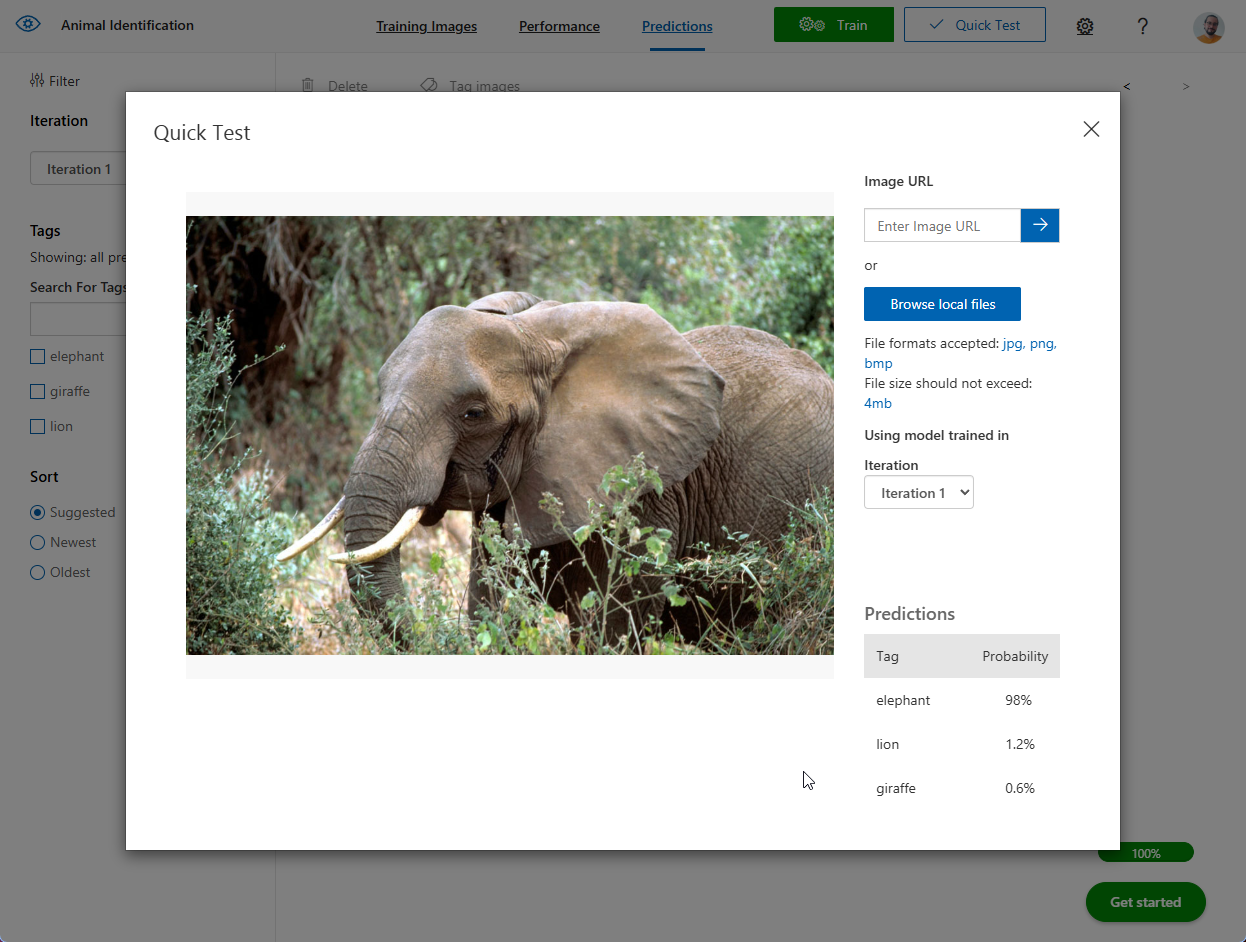
\includegraphics[width=0.48\linewidth]{assets/images/fig_qt_elephant1.png}
    \hfill
    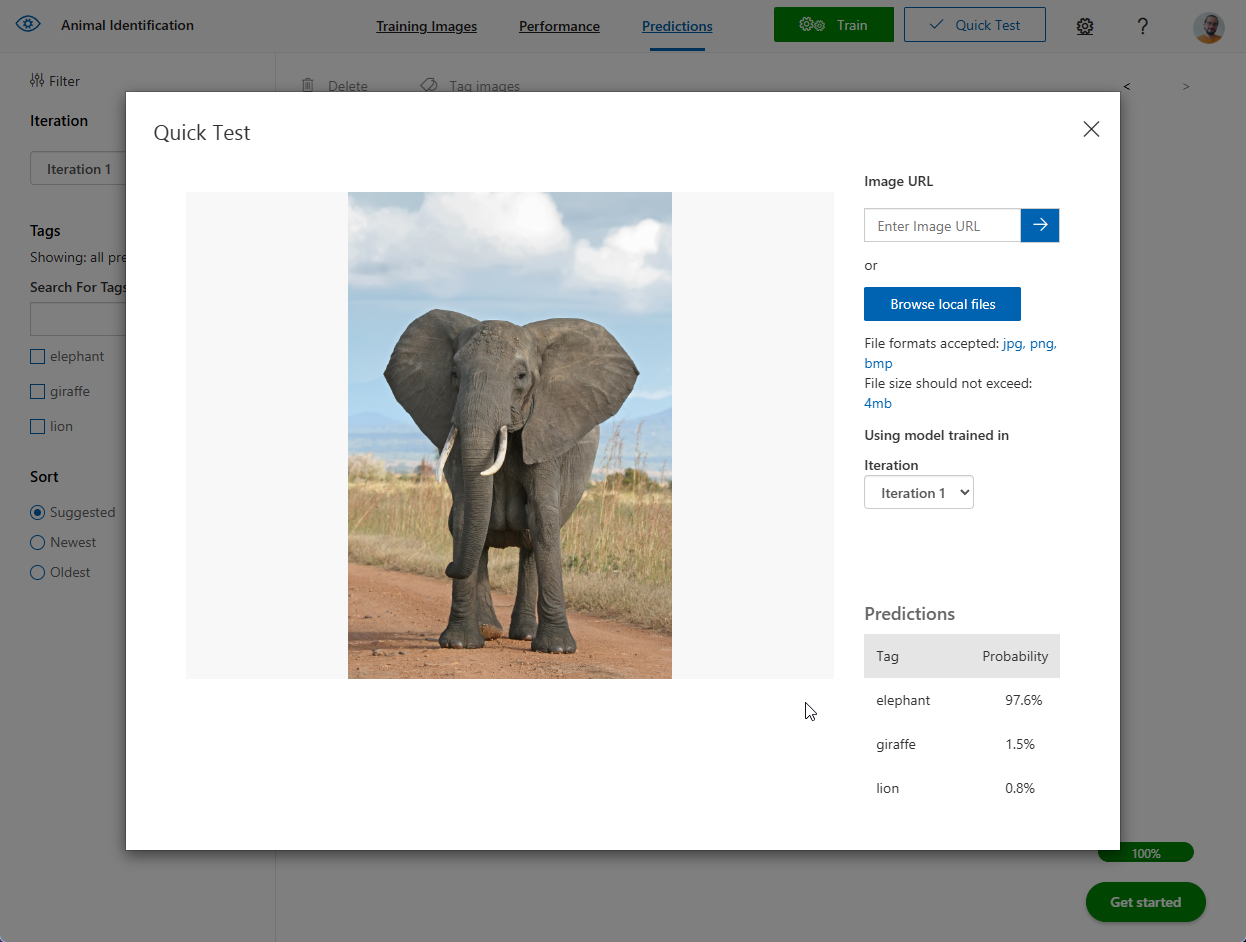
\includegraphics[width=0.48\linewidth]{assets/images/fig_qt_elephant2.png}
    \caption{Quick Test en elefantes nuevos: 98.0\% y 97.6\%.}
    \label{fig:qt1}
  \end{figure}

  \begin{figure}[H]
    \centering
    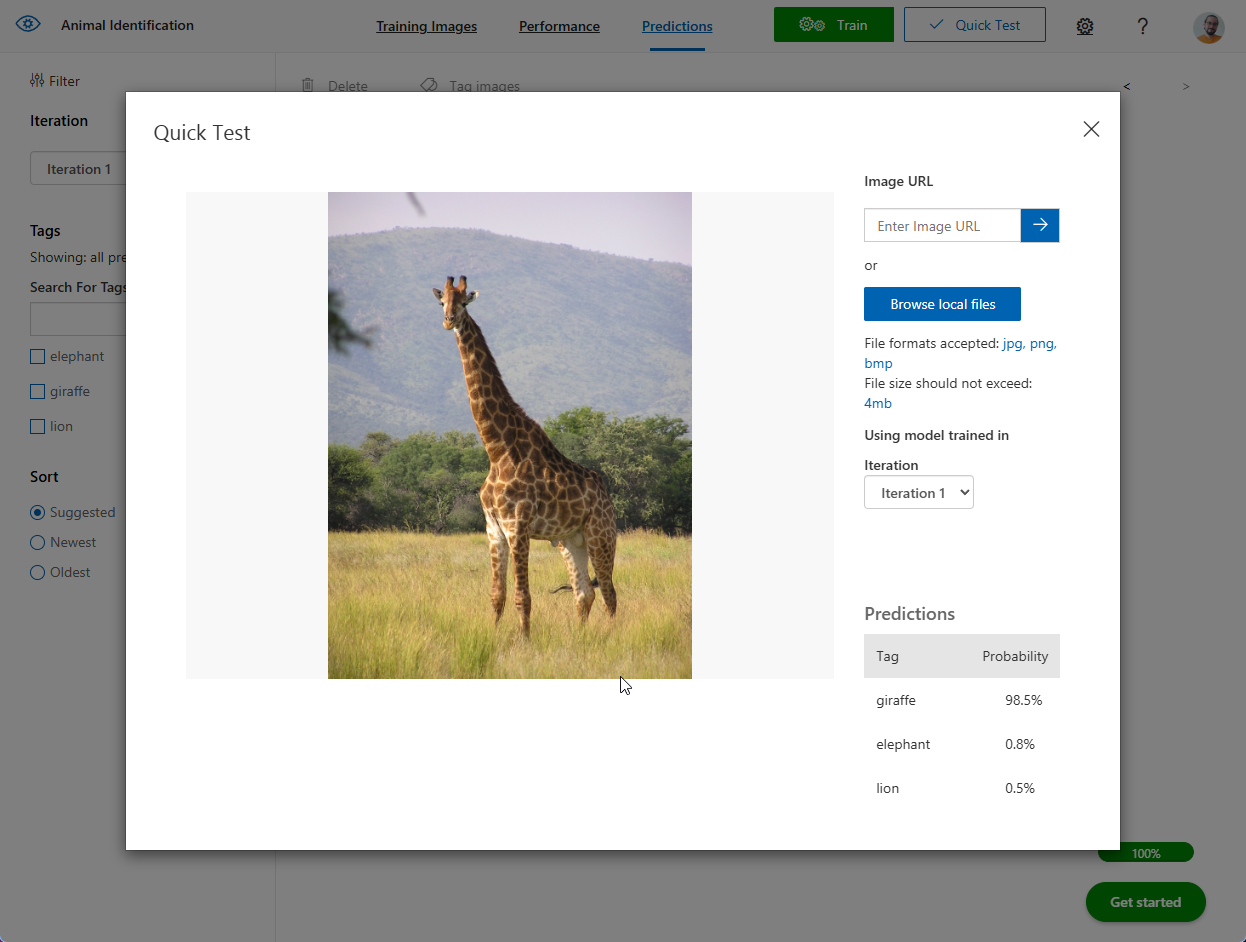
\includegraphics[width=0.48\linewidth]{assets/images/fig_qt_giraffe1.png}
    \hfill
    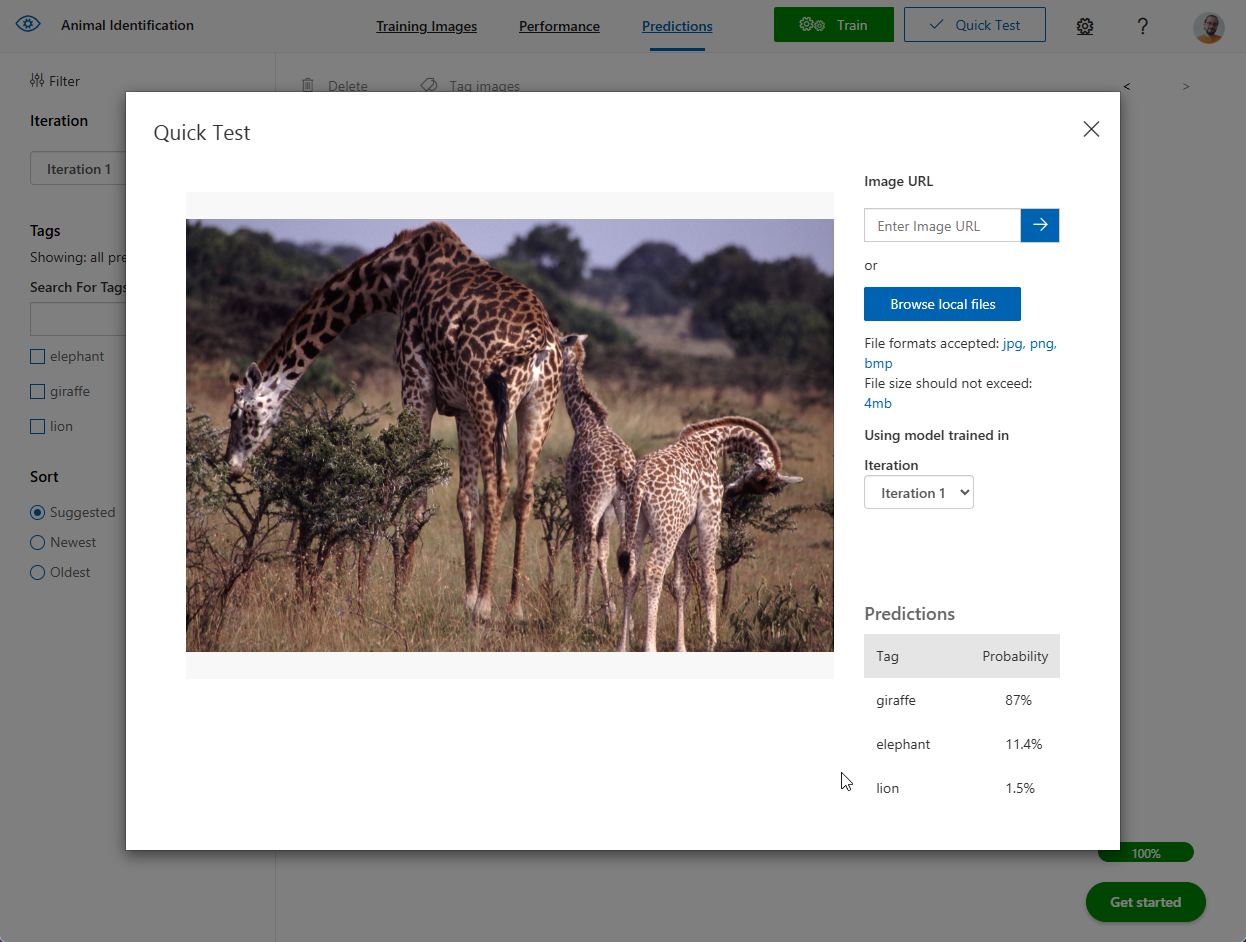
\includegraphics[width=0.48\linewidth]{assets/images/fig_qt_giraffe2.png}
    \caption{Quick Test en jirafas nuevas: 98.5\% y 87.0\% (tres ejemplares con oclusi\'on).}
    \label{fig:qt2}
  \end{figure}

  \begin{figure}[H]
    \centering
    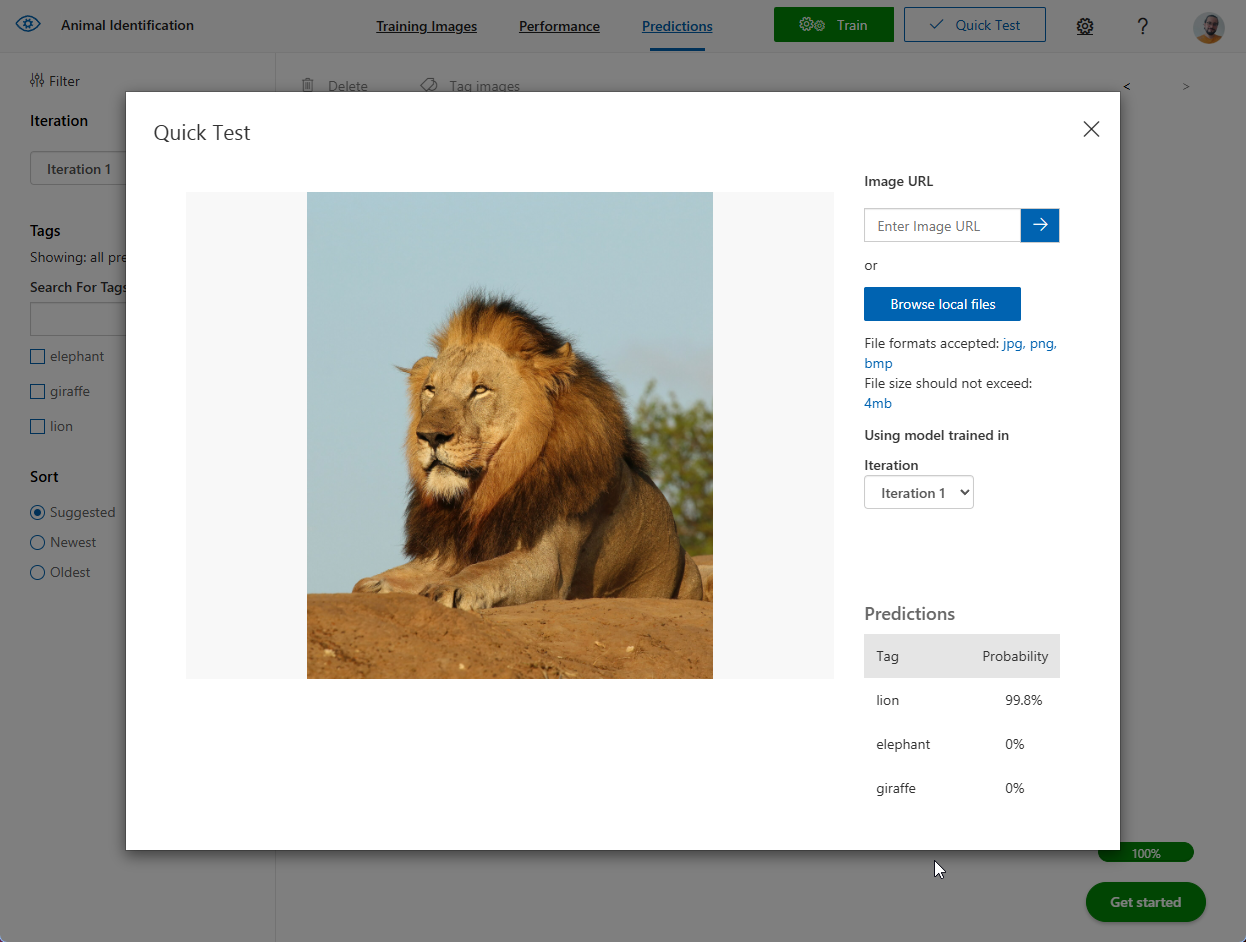
\includegraphics[width=0.48\linewidth]{assets/images/fig_qt_lion1.png}
    \hfill
    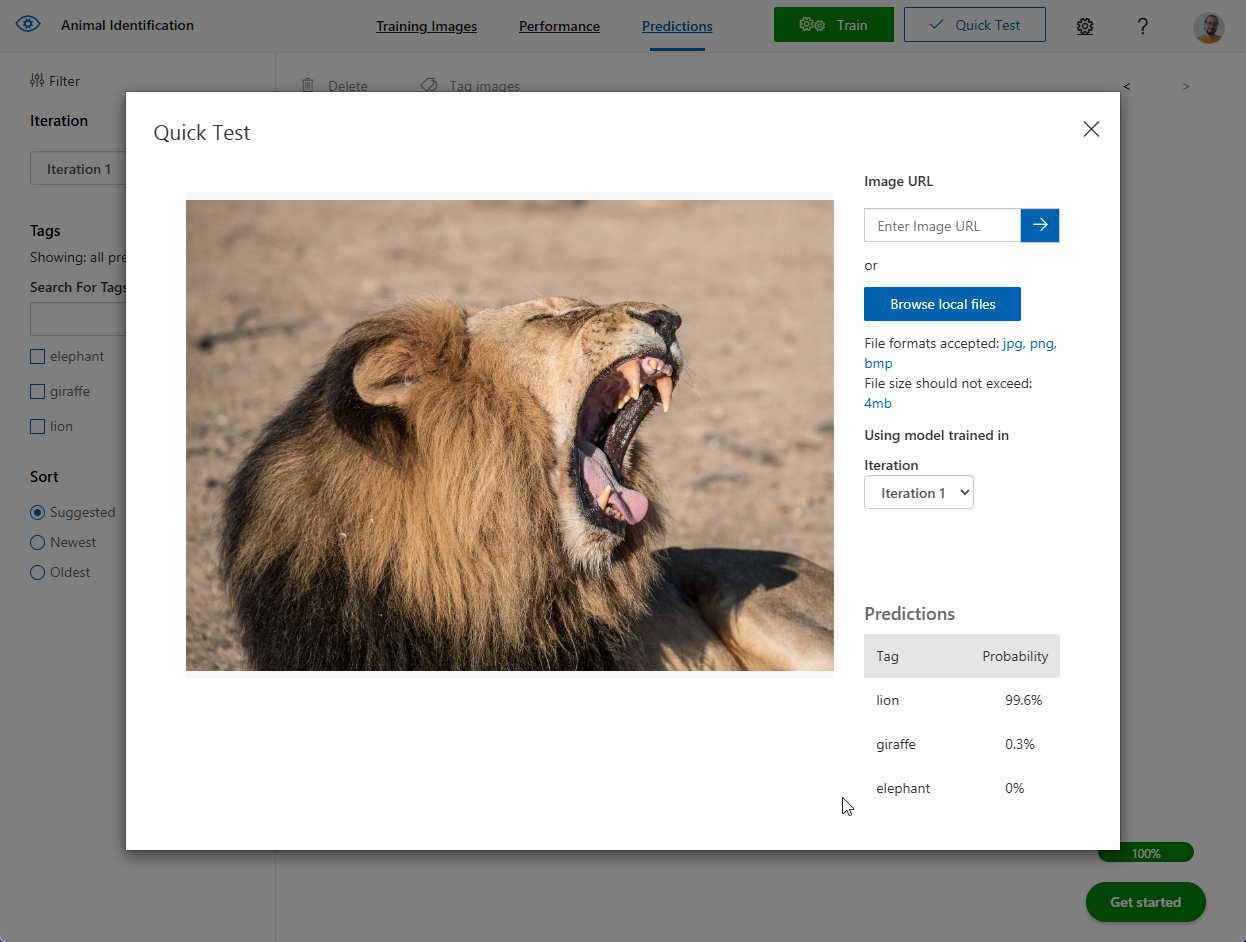
\includegraphics[width=0.48\linewidth]{assets/images/fig_qt_lion2.png}
    \caption{Quick Test en leones nuevos: 99.8\% y 99.6\%.}
    \label{fig:qt3}
  \end{figure}

  \section{Publicaci\'on y Cliente}

  La Iteraci\'on 1 se public\'o como modelo \texttt{AnimalIdentification-v1} contra el recurso \texttt{labunisalle-Prediction} en \texttt{northcentralus}. El endpoint de imagen es:

  \begin{lstlisting}
https://labunisalle-prediction.cognitiveservices.azure.com/
customvision/v3.0/Prediction/8745a5dd-92de-4fd7-967f
-642ce3967c6c/classify/iterations/Iteration1/image
  \end{lstlisting}

  con headers \texttt{Prediction-Key: <clave del portal>} y \texttt{Content-Type: application/octet-stream}. La clave completa queda guardada en el portal (\texttt{labunisalle-Prediction > Keys and Endpoint}) y no se imprime en este PDF por seguridad; se rota despu\'es de la entrega.

  La prueba del cliente se hizo con \texttt{curl} sobre dos im\'agenes de validaci\'on no vistas (salida completa en \texttt{capturas/14-cloudshell-test.txt}):

  \begin{lstlisting}
$ curl -s -X POST "$PREDICT_URL_IMAGE" \
  -H "Prediction-Key: $PKEY" \
  -H "Content-Type: application/octet-stream" \
  --data-binary "@validacion/lion/lion_val_01.jpg"
lion 0.9986, elephant 0.0008, giraffe 0.0005
$ curl -s -X POST "$PREDICT_URL_IMAGE" \
  --data-binary "@validacion/giraffe/giraffe_val_02.jpg"
giraffe 0.8700, elephant 0.1147, lion 0.0153
  \end{lstlisting}

  Los valores coinciden con el Quick Test del portal (99.8\% y 87.0\%), as\'i que el modelo publicado responde igual que el evaluado.

  \section{Limitaciones}

  La principal limitaci\'on no es del modelo sino de la suscripci\'on: la policy regional impide seguir literalmente el instructivo en \texttt{East US} y obliga a \texttt{northcentralus}. El dominio General disponible en esa regi\'on puede diferir en nombre de \texttt{General [A2]}; se deja constancia del valor exacto elegido. El conjunto es peque\~no (51 im\'agenes), as\'i que las m\'etricas describen este ejercicio y no generalizan.

  \bibliographystyle{IEEEtran}
  \bibliography{bib/references}

\end{document}
